\documentclass{article}

\usepackage[utf8]{inputenc}
\usepackage[portuguese]{babel}
\usepackage{blindtext}
\usepackage{graphicx}
\usepackage{amsmath}
\usepackage{float}
\usepackage{caption}
\usepackage[compact]{titlesec}
\usepackage{multicol}
\usepackage[a4paper, total={7.5in, 10in}]{geometry}
\usepackage[font=scriptsize,labelfont=bf]{caption}
\usepackage{listings}
\usepackage{color}
 
\definecolor{codegreen}{rgb}{0,0.6,0}
\definecolor{codegray}{rgb}{0.5,0.5,0.5}
\definecolor{codepurple}{rgb}{0.58,0,0.82}
\definecolor{backcolour}{rgb}{0.95,0.95,0.92}
 
\lstdefinestyle{mystyle}{
    backgroundcolor=\color{backcolour},   
    commentstyle=\color{codegreen},
    keywordstyle=\color{magenta},
    numberstyle=\tiny\color{codegray},
    stringstyle=\color{codepurple},
    basicstyle=\footnotesize,
    breakatwhitespace=false,         
    breaklines=true,                 
    captionpos=b,                    
    keepspaces=true,                 
    numbers=left,                    
    numbersep=5pt,                  
    showspaces=false,                
    showstringspaces=false,
    showtabs=false,                  
    tabsize=2
}
 
\lstset{style=mystyle}

\setlength{\columnsep}{1cm}
\setlength{\parindent}{0em}
\titlespacing{\section}{1pt}{*0.5}{*0.5}
\begin{document}

\textbf{Relatório de Entrega de Trabalho} \newline
\textbf{Disciplina de Programação Paralela (PP)}\textbf{ - Prof. César De Rose} \newline
\textbf{Alunos:} Rafael Rios e Rodrigo Silveira \newline
\textbf{Exercício:} TPP2: MPI Divisão e Conquista (D&C) \newline

\begin{multicols*}{2}

\section{Implementação}
O objetivo deste trabalho foi implementar um algoritmo de divisão e conquista para compreender aplicações paralelas, usando a biblioteca MPI. O problema proposto consiste em ordenar um vetor de 1000000 elementos, originalmente em ordem decrescente, para ordem crescente, utilizando o algoritmo bubblesort e quicksort. A estrutura de processos baseia-se em uma árvore binária balanceada, executando o algoritmo para um número de processos que seja "potência de dois menos um" (1, 3, 7, 15, 31), de modo a garantir a estrutura proposta onde todos nodos pais tem dois filhos, o algoritmo foi executado para três casos com o intuito de mostrar as diferenças nos tempos de ordenamento. O primeiro teste caracterizou-se pelo pai dividir o vetor igualmente para os filhos até os filhos receberem o vetor com um tamanho menor ou igual a um delta pré estabelecido conforme o número de processos, sendo executado até 31 nodos (HT), em um segundo momento, o algoritmo foi testado para um número de processos maiores que o Hyper-Threading e por último, realizou-se alterações no código para os pais ordenarem uma parte do vetor e dividir o resto para os filhos, com a finalidade de melhor ainda mais o tempo de execução. \newline
Como foi explicado, o algoritmo paralelo divide o vetor até o mesmo ser conquistado e ordenado pelos filhos, no inicio, o processo 0 cria o vetor enquanto os outros aguardam o recebimento do mesmo junto com a mensagem do tamanho do vetor recebido (MPI\_Get\_count). O processamento do que é feito com o vetor é realizado de modo igual por todos os processos no código, caso o tamanho do vetor recebido seja menor ou igual ao delta pré estabelecido, o vetor é ordenado, caso contrário, o vetor é separado e enviado para os filhos, que são escolhidos pelas fórmulas 2*(rank do processo)+1 e 2*(rank do processo)+2, garantindo a sequência na ordem dos processos. Outra implementação foi o controle para tamanhos de vetor não divisíveis por dois (Ex: 15625), quando isso ocorre, o filho da esquerda recebe a metade do vetor truncada (Ex: 7812) e o da direita a metade do vetor arredondada por excesso (Ex: 7813), esse controle é feito comparando o tamanho do vetor que os filhos receberão (float), com esse tamanho +0.5 truncado (int), caso for igual, ele é divisível por dois, caso contrário deve ser dividido como foi explicado. O mesmo código foi usado para a execução do algoritmo ordenado localmente pelos pais, antes de demonstrar o seu funcionamento, deve-se explicar duas variáveis: "tam\_local" é o tamanho que será executado localmente pelo pai e "tam\_divide" que é o tamanho a ser dividido igualmente pelos filhos, o controle é feito através de um valor definido (LOCAL), se for local, "tam\_local" recebe delta e "tam\_divide" recebe o tamanho do vetor subtraído pelo delta, se não for local, "tam\_local" recebe zero e "tam\_divide" recebe todo o tamanho do vetor a ser dividido. Após o envio do vetor para os filhos, se for o algoritmo com execução local, ele ordena a sua parte do vetor, depois, o pai recebe o vetor ordenado dos filhos (levando em conta se o tamanho enviado era divisível por dois) e organiza-o de modo a ficar ordenado, mostrando o tempo de execução no final, pelo processo 0.

\section{Dificuldades encontradas}
Elaboração de um método para garantir a ordem certa de envio dos vetores para os filhos, escolhendo quais processos receberiam o vetor; Resolução do problema para quando o tamanho do vetor não seria divisível por dois.

\section{Testes}
Foram realizados testes com alocação de 2 nodos na grad, executando o algoritmo de divisão e conquista para 7, 15, 31, 63, 127 e 255 processos, adquirindo o tempo de processamento e o tempo levando em conta a instanciação dos processos. O tempo do código sequencial (1 processo) e o tempo para 3 processos foram disponibilizados, sendo, respectivamente, 4440 segundos e 1080 segundos.

\section{Análise de desempenho}
Para o algoritmo quicksort, não houve uma mudança significativa nos tempos medidos, já que o algoritmo apresenta uma execução muito mais rápido. Entretanto, para o algoritmo bubblesort, notou-se que conforme aumentava-se o número de processos em potência de dois, o tempo de execução praticamente diminuía pela metade, mesmo passando do ponto de HT (pós 31 processos). Portanto, o speed-up também aumentava a cada execução, passando do ideal e demonstrando o grande aumento de desempenho da execução paralela em relação à sequencial, a eficiência também ficou acima do ideal, todavia estabilizando por volta de 4.0 após 15 processos para a ordenação nos últimos filho e em 13.0 para o algoritmo com execução local, também após 15 processos.

\section{Observações Finais}
TBD\newline
A utilização do modelo mestre/escravo se mostrou eficiente para os algoritmos tanto do quicksort quanto do bubblesort com a carga de 1.000 vetores de 100.000 valores no caso do quicksort e de 1.000 vetores de 10.000 valores no caso do bubblesort. Obteve-se um speedup significativo ao se comparar as versões paralelas às sequenciais. Também foi possível perceber a degradação do desempenho ao ultrapassar um certo número de processos, devido ao overhead da troca de mensagens e pelo gargalo ocasionado pelo fato de todo processamento ter que ser gerenciado pelo único processo mestre. Não obstante, para um número tanto pequeno quanto elevado de processos, os tempos de execução dos códidos paralelos foram consideravelmente menores que os tempo dos códigos sequenciais.

\end{multicols*}

\newpage

\begin{figure}[H]
            \centering
            \vspace{-0.3em}
            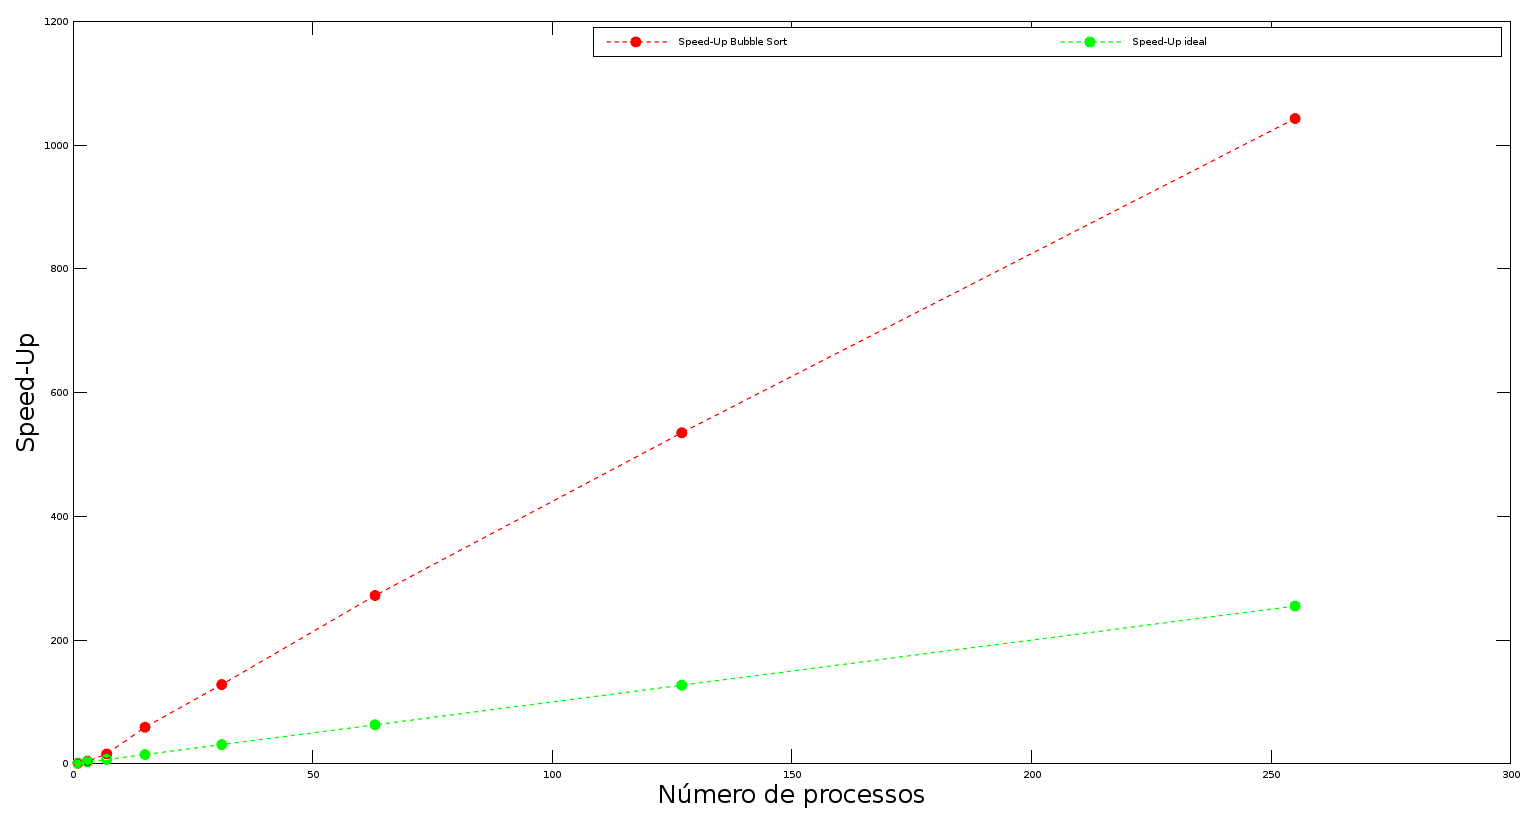
\includegraphics[width=14cm, height=7cm]{sup.png}
            \vspace{-0.6em}
            \caption{Gráfico com Speed-Up}
            \vspace{-1.1em}
\end{figure}

\begin{figure}[H]
            \centering
            \vspace{-0.3em}
            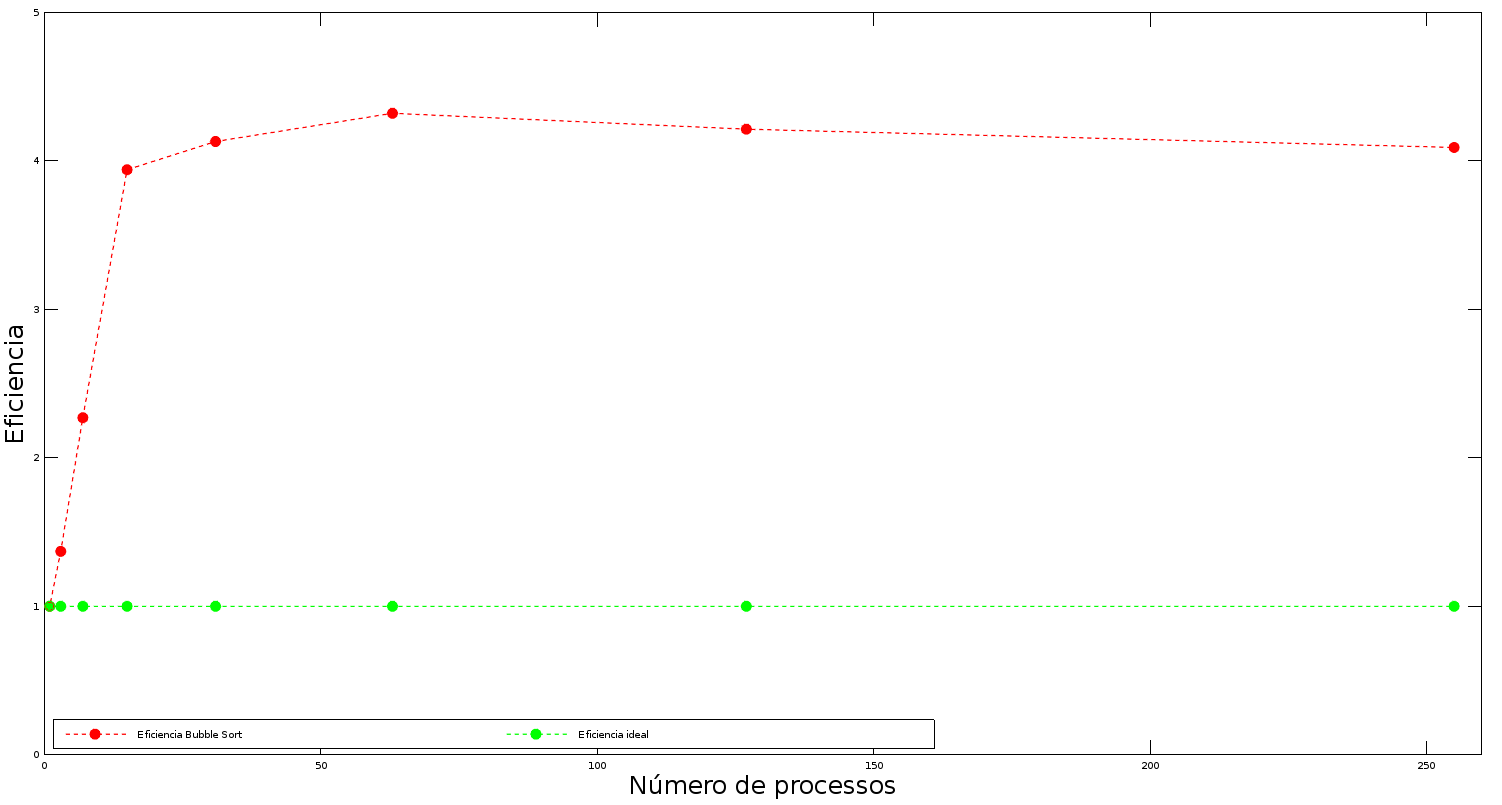
\includegraphics[width=14cm, height=7cm]{eficiencia.png}
            \vspace{-0.6em}
            \caption{Gráfico com Eficiência}
            \vspace{-1.1em}
\end{figure}

\begin{figure}[H]
            \centering
            \vspace{-0.3em}
            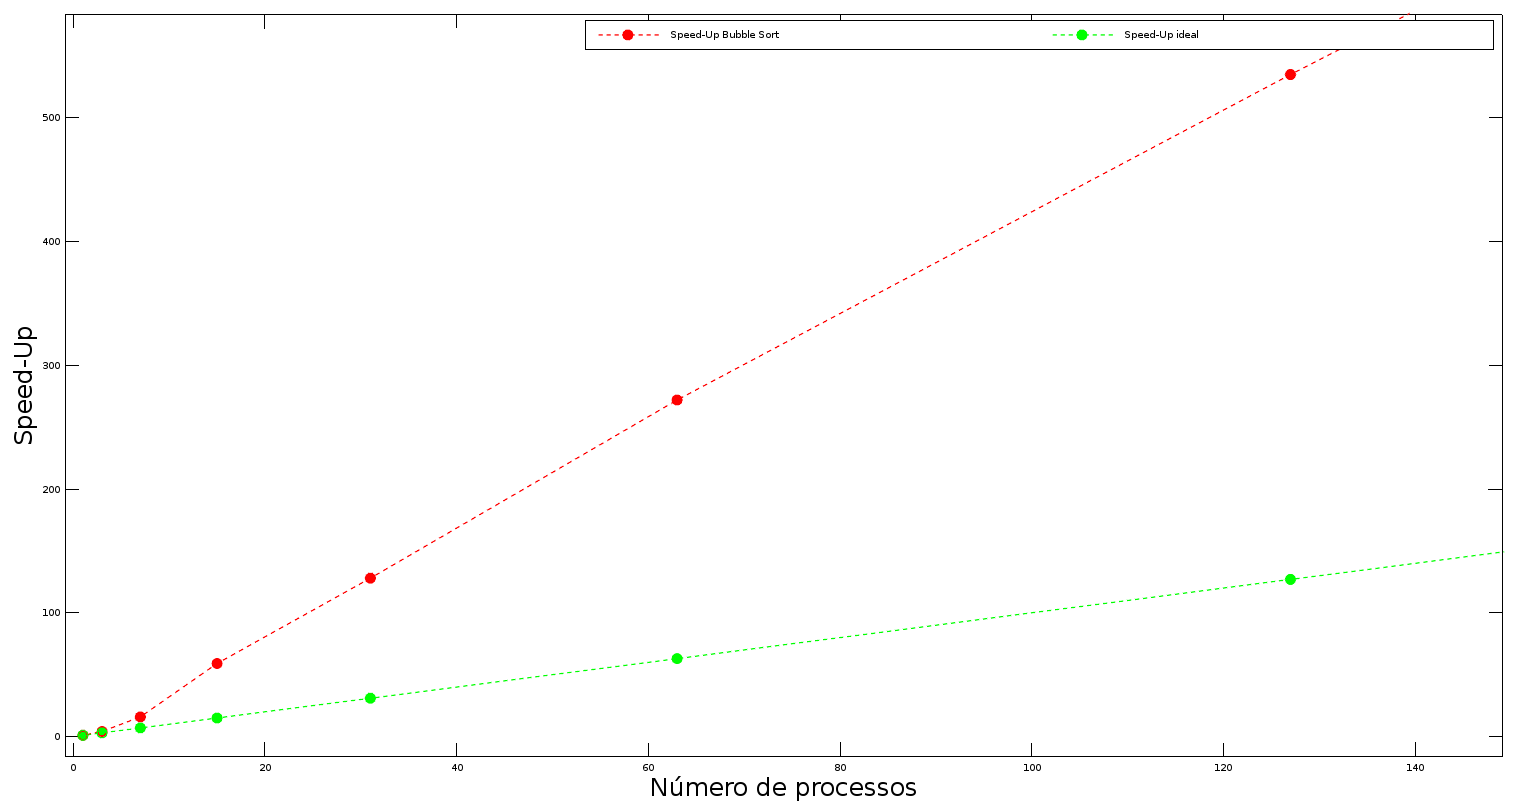
\includegraphics[width=14cm, height=7cm]{sup_close.png}
            \vspace{-0.6em}
            \caption{Valores calculados}
            \vspace{-1.1em}
\end{figure}
\newpage

\lstinputlisting[language=C++]{tpp2.c}

\end{document}
